\documentclass[11pt]{article}

\usepackage[margin=1in]{geometry}
\usepackage{amsmath, amssymb, amsfonts}
\usepackage{booktabs}
\usepackage{graphicx}
\usepackage[hidelinks,hypertexnames=false]{hyperref}
\usepackage{natbib}
\usepackage{float}
\usepackage{placeins}

\setlength{\textfloatsep}{8pt plus 2pt minus 2pt}
\setlength{\intextsep}{8pt plus 2pt minus 2pt}
\setlength{\floatsep}{8pt plus 2pt minus 2pt}
\setlength{\abovecaptionskip}{4pt plus 1pt minus 1pt}
\setlength{\belowcaptionskip}{2pt plus 1pt minus 1pt}

\graphicspath{{../reports/figures/}}
\newcommand{\ETFUniverseTable}{%
\begin{table}[H]
\centering
\caption{ETF universe and modeling roles. BIL is used only as the cash proxy.}
\label{tab:etf_universe}
\resizebox{\linewidth}{!}{%
\begin{tabular}{llllll}
\toprule
Group & Tickers & Role & Alpha & Covariance & Cash Sleeve \\
\midrule
Equity & SPY, QQQ, IWM, EFA, EEM & Risky ETF & Yes & Yes & No \\
Treasury & TLT, IEF, SHY & Risky ETF & Yes & Yes & No \\
Credit & LQD, HYG & Risky ETF & Yes & Yes & No \\
Real Assets & GLD, DBC, VNQ & Risky ETF & Yes & Yes & No \\
Cash & BIL & Cash proxy & No & No & Yes \\
\bottomrule
\end{tabular}
}
\end{table}

}
\newcommand{\MainPerformanceTable}{%
\begin{table}[H]
\centering
\caption{Main performance summary using net returns after transaction costs.}
\label{tab:main_performance}
\resizebox{\linewidth}{!}{%
\begin{tabular}{lrrrrrrrrr}
\toprule
Strategy & Ann. Return & Ann. Vol. & Sharpe & Max DD & Calmar & Final NV & Avg TO & Cost Drag & Avg Cash \\
\midrule
Equal Weight & 6.9\% & 9.5\% & 0.75 & -20.7\% & 0.34 & 2.73 & 1.7\% & 0.02\% & 0.0\% \\
Minimum Variance & 3.1\% & 4.3\% & 0.73 & -14.6\% & 0.21 & 1.59 & 3.4\% & 0.04\% & 0.0\% \\
Traditional MVO & 9.2\% & 12.1\% & 0.79 & -19.6\% & 0.47 & 3.74 & 19.0\% & 0.25\% & 0.0\% \\
Proposed Strategy & 9.8\% & 10.2\% & 0.96 & -15.7\% & 0.62 & 4.04 & 27.7\% & 0.37\% & 9.8\% \\
\bottomrule
\end{tabular}
}
\end{table}

}
\newcommand{\DrawdownSummaryTable}{%
\begin{table}[H]
\centering
\caption{Maximum drawdown periods for the four main strategies.}
\label{tab:drawdown_summary}
\resizebox{\linewidth}{!}{%
\begin{tabular}{lrrrrr}
\toprule
Strategy & Max DD & Start & Valley & Recovery & Days \\
\midrule
Equal Weight & -20.7\% & 2021-11-09 & 2022-10-14 & 2024-06-18 & 952 \\
Minimum Variance & -14.6\% & 2021-09-15 & 2022-10-20 & 2024-09-19 & 1100 \\
Traditional MVO & -19.6\% & 2018-01-26 & 2018-12-24 & 2020-01-16 & 720 \\
Proposed Strategy & -15.7\% & 2020-02-19 & 2020-03-19 & 2020-07-29 & 161 \\
\bottomrule
\end{tabular}
}
\end{table}

}
\newcommand{\SignalRiskDiagnosticsTable}{%
\begin{table}[H]
\centering
\caption{Signal and risk-forecast diagnostics for the proposed strategy.}
\label{tab:signal_risk_diagnostics}
\begin{tabular}{lr}
\toprule
Diagnostic & Value \\
\midrule
Average cross-sectional IC & 0.072 \\
IC standard deviation & 0.458 \\
IC t-statistic & 2.11 \\
IC during normal periods & 0.088 \\
IC during drawdown periods & 0.015 \\
Positive IC ratio & 55.3\% \\
Average predicted volatility & 8.2\% \\
Average target volatility & 11.8\% \\
Average realized 21-day volatility & 9.3\% \\
Average realized/predicted ratio & 1.28 \\
Target-volatility binding rate & 28.3\% \\
\bottomrule
\end{tabular}
\end{table}

}
\newcommand{\TargetVolSensitivityTable}{%
\begin{table}[H]
\centering
\caption{Target-volatility sensitivity for the proposed strategy.}
\label{tab:target_vol_sensitivity}
\resizebox{\linewidth}{!}{%
\begin{tabular}{lrrrrrrr}
\toprule
Target Volatility & Ann. Return & Ann. Vol. & Sharpe & Max DD & Calmar & Avg Cash & Avg TO \\
\midrule
6.0\% & 8.5\% & 8.6\% & 0.99 & -13.4\% & 0.63 & 18.7\% & 35.0\% \\
8.0\% & 9.5\% & 9.6\% & 0.98 & -14.2\% & 0.66 & 12.9\% & 31.1\% \\
10.0\% & 9.8\% & 10.2\% & 0.96 & -15.7\% & 0.62 & 9.8\% & 27.7\% \\
12.0\% & 9.6\% & 10.6\% & 0.92 & -16.5\% & 0.58 & 8.1\% & 26.3\% \\
\bottomrule
\end{tabular}
}
\end{table}

}
\newcommand{\AlphaScaleSensitivityTable}{%
\begin{table}[H]
\centering
\caption{Alpha-scale sensitivity for the proposed strategy.}
\label{tab:alpha_scale_sensitivity}
\resizebox{\linewidth}{!}{%
\begin{tabular}{lrrrrrrr}
\toprule
Alpha Scale & Ann. Return & Ann. Vol. & Sharpe & Max DD & Calmar & Avg Cash & Avg TO \\
\midrule
1.0\% & 9.3\% & 9.3\% & 1.00 & -13.8\% & 0.68 & 15.9\% & 27.1\% \\
2.0\% & 9.4\% & 10.0\% & 0.95 & -15.1\% & 0.63 & 11.0\% & 27.5\% \\
3.0\% & 9.8\% & 10.2\% & 0.96 & -15.7\% & 0.62 & 9.8\% & 27.7\% \\
5.0\% & 10.1\% & 10.4\% & 0.98 & -17.0\% & 0.59 & 9.0\% & 28.2\% \\
\bottomrule
\end{tabular}
}
\end{table}

}
\newcommand{\RhoSensitivityTable}{%
\begin{table}[H]
\centering
\caption{Robust penalty sensitivity for the proposed strategy.}
\label{tab:rho_sensitivity}
\resizebox{\linewidth}{!}{%
\begin{tabular}{lrrrrrr}
\toprule
Rho Setting & Ann. Return & Ann. Vol. & Sharpe & Max DD & Calmar & Avg Cash \\
\midrule
rho\_multiplier=0 & 10.2\% & 10.5\% & 0.98 & -19.3\% & 0.53 & 8.9\% \\
rho\_multiplier=0.5 & 10.2\% & 10.4\% & 0.98 & -17.5\% & 0.58 & 9.2\% \\
rho\_multiplier=1 & 9.8\% & 10.2\% & 0.96 & -15.7\% & 0.62 & 9.8\% \\
rho\_multiplier=1.5 & 9.5\% & 10.1\% & 0.95 & -14.7\% & 0.64 & 10.5\% \\
rho\_multiplier=2 & 9.5\% & 10.0\% & 0.96 & -14.7\% & 0.64 & 11.3\% \\
\bottomrule
\end{tabular}
}
\end{table}

}
\newcommand{\CovarianceSensitivityTable}{%
\begin{table}[H]
\centering
\caption{Covariance estimator sensitivity. Ledoit-Wolf is a robustness case, not the final implemented risk model.}
\label{tab:covariance_sensitivity}
\resizebox{\linewidth}{!}{%
\begin{tabular}{lrrrrrrr}
\toprule
Estimator & Ann. Return & Ann. Vol. & Sharpe & Max DD & Calmar & Avg Cash & Real./Pred. \\
\midrule
Sample Covariance & 9.8\% & 10.2\% & 0.97 & -16.2\% & 0.60 & 10.2\% & 1.21 \\
Ledoit-Wolf Shrinkage & 10.2\% & 10.4\% & 0.98 & -15.1\% & 0.67 & 9.7\% & 1.31 \\
Final Implemented Covariance Method & 9.8\% & 10.2\% & 0.96 & -15.7\% & 0.62 & 9.8\% & 1.25 \\
\bottomrule
\end{tabular}
}
\end{table}

}
\newcommand{\TransactionCostSensitivityTable}{%
\begin{table}[H]
\centering
\caption{Transaction-cost sensitivity for the proposed strategy.}
\label{tab:transaction_cost_sensitivity}
\resizebox{\linewidth}{!}{%
\begin{tabular}{lrrrrrr}
\toprule
Cost Rate & Ann. Return & Ann. Vol. & Sharpe & Max DD & Ann. Cost Drag & Final NV \\
\midrule
0 bps & 10.1\% & 10.2\% & 1.00 & -15.7\% & 0.00\% & 4.25 \\
5 bps & 10.0\% & 10.2\% & 0.98 & -15.7\% & 0.18\% & 4.14 \\
10 bps & 9.8\% & 10.2\% & 0.96 & -15.7\% & 0.37\% & 4.04 \\
25 bps & 9.2\% & 10.2\% & 0.92 & -15.8\% & 0.91\% & 3.75 \\
\bottomrule
\end{tabular}
}
\end{table}

}
\newcommand{\ImplementationChecksTable}{%
\begin{table}[H]
\centering
\caption{Constraint, solver, and no-look-ahead implementation checks.}
\label{tab:implementation_checks}
\begin{tabular}{lr}
\toprule
Check & Value \\
\midrule
Max budget violation & 2.22e-16 \\
Max long-only violation & 0.00e+00 \\
Max upper-bound violation & 2.26e-10 \\
Max target-volatility violation & 4.95e-10 \\
Solver failures & 0 \\
Fallback uses & 0 \\
Rebalance dates & 180 \\
Timing checks passed & 5/5 \\
\bottomrule
\end{tabular}
\end{table}

}
\newcommand{\MethodologyCodeConsistencyTable}{%
\begin{table}[H]
\centering
\caption{Methodology-code consistency checklist for the final proposed strategy.}
\label{tab:methodology_code_consistency}
\resizebox{\linewidth}{!}{%
\begin{tabular}{ll}
\toprule
Item & Implemented value \\
\midrule
$\alpha_{scale}$ & 0.03 \\
EWMA covariance decay & 0.94 \\
Transaction cost rate & 0.001 per one-way turnover \\
L2 concentration penalty & 0.01 \\
$v_t$ & $\operatorname{clip}(\sigma^{EW,EWMA20}_t / \sigma^{EW,252}_t,0.5,2.5)$ \\
$\rho_t$ & $\operatorname{clip}(0.08v_t,0.03,0.25)$ \\
$\sigma_t^*$ & $\operatorname{clip}(0.10/v_t,0.04,0.16)$ \\
Single-ETF upper bound & 0.25 \\
Cash proxy & BIL \\
BIL in alpha/covariance & Excluded from both \\
\bottomrule
\end{tabular}
}
\end{table}

}


\title{A Cash-Allowed Robust Forecast-Aware Portfolio Optimization Framework for Multi-Asset ETF Allocation}
\author{Junyuan Ding}
\date{}

\begin{document}

\maketitle

\begin{abstract}
This paper develops a cash-allowed robust forecast-aware portfolio optimization
framework for multi-asset ETF allocation. Traditional mean-variance optimization
remains a foundational approach to portfolio construction, but its practical
performance is often fragile because expected returns and covariances are difficult
to estimate. The research question is whether interpretable forecast signals and
convex risk controls can improve allocation behavior relative to standard portfolio
rules. The proposed model constructs expected-return forecasts from 12-1 momentum
and 200-day trend signals, estimates risk with annualized 20-day EWMA covariance
and positive-semidefinite repair, incorporates a robust penalty for forecast
uncertainty, includes a BIL cash sleeve, controls implementation cost through
full-vector turnover, and imposes a dynamic target-risk budget. Monthly rolling
out-of-sample backtests compare the proposed strategy with Equal Weight, Minimum
Variance, and Traditional MVO baselines. In the tested sample, the proposed strategy
achieves a 9.8\% annualized net return, 10.2\% annualized volatility, a Sharpe ratio
of 0.96, and a maximum drawdown of -15.7\%, compared with Sharpe ratios of 0.75,
0.73, and 0.79 for Equal Weight, Minimum Variance, and Traditional MVO. The results
suggest that robust forecast-aware optimization with an explicit cash sleeve can
improve certain risk-adjusted metrics in this ETF universe, although performance
remains dependent on forecast quality, volatility estimation, transaction-cost
assumptions, and market regimes.
\end{abstract}

\section{Introduction}

Asset allocation is a central problem for investors who allocate capital across
equities, government bonds, credit, real assets, and cash-like instruments. Exchange
traded funds make this problem especially relevant because they provide liquid and
diversified exposure to broad asset classes. Unlike single-stock selection, a
multi-asset ETF allocation problem naturally emphasizes portfolio-level properties:
return, volatility, drawdown, turnover, and implementation cost. A useful allocation
framework should therefore be evaluated not only by cumulative return, but also by
risk-adjusted performance, exposure dynamics, and trading frictions.

Markowitz mean-variance optimization provides the classical framework for balancing
expected return and risk \citep{markowitz1952}. Its practical implementation,
however, is sensitive to estimation error. Expected returns are especially noisy,
finite-sample covariance matrices may be unstable, and optimized weights can become
extreme when the optimizer exploits estimation noise. A fully invested risky-asset
model is also unable to reduce aggregate risky exposure during market stress unless
cash is explicitly included as an allocation choice. These issues help explain why
simple allocation rules such as equal weighting remain important benchmarks in
empirical portfolio research.

This paper studies a forecast-aware but conservative alternative. Price-based
momentum and trend variables may contain useful information about relative expected
returns across asset classes, but their predictive ability is imperfect and
regime-dependent. The proposed strategy therefore does not use momentum as a
standalone ranking rule. Instead, momentum and trend signals are converted into an
annualized alpha vector that enters a convex robust optimization problem. The
optimizer balances forecasted alpha against EWMA risk, robust forecast uncertainty,
concentration regularization, transaction costs, and a dynamic target-risk budget.

The proposed model allocates across a risky ETF universe and a BIL cash sleeve. The
risky ETF universe includes equity, Treasury, credit, and real asset ETFs, while BIL
is used only as a cash proxy. The final strategy uses annualized 20-day EWMA
covariance estimation with positive-semidefinite repair, a volatility-adaptive robust
penalty, a dynamic risk budget based on recent market stress, full-vector turnover
costs, and monthly rolling out-of-sample backtesting. The model remains a convex
optimization problem and is implemented with a second-order-cone-compatible risk
term.

The paper makes three contributions. First, it integrates medium-term momentum and
trend forecasts into a robust convex optimization framework for multi-asset ETF
allocation. Second, it allows cash allocation through an explicit BIL sleeve, so the
optimizer is not forced to remain fully invested in risky assets. Third, it evaluates
the strategy using cumulative performance, drawdown, Sharpe and Sortino ratios, cash
and group exposure, signal diagnostics, volatility forecast diagnostics, turnover,
transaction-cost drag, and parameter sensitivity tests. The remainder of the paper is
organized as follows. Section \ref{sec:literature} reviews related literature.
Section \ref{sec:data} describes the ETF universe and data construction. Section
\ref{sec:methodology} presents the methodology. Section \ref{sec:baselines} defines
the baselines. Sections \ref{sec:results} through \ref{sec:robustness} report the
empirical results, diagnostics, and robustness analysis. Section \ref{sec:discussion}
discusses limitations, and Section \ref{sec:conclusion} concludes.

\section{Literature Review}
\label{sec:literature}

\subsection{Mean-Variance Optimization and Estimation Error}

The starting point is the mean-variance framework of \citet{markowitz1952}, which
formalizes portfolio selection as a tradeoff between expected return and variance.
The framework is theoretically elegant, but its empirical performance depends on
estimated inputs. \citet{demiguel2009} show that naive \(1/N\) diversification is a
difficult benchmark to beat after accounting for estimation error. This evidence
motivates the inclusion of Equal Weight as a primary baseline. Covariance estimation
error is another important source of instability. \citet{ledoitwolf2004} propose
covariance shrinkage to improve conditioning, while \citet{jagannathanma2003} show
that portfolio constraints such as no-short-sale restrictions can reduce effective
estimation error and act as implicit regularization. In the present paper,
Ledoit-Wolf shrinkage is discussed as background and as a covariance sensitivity
case; the final implemented proposed strategy uses EWMA covariance estimation with
positive-semidefinite repair.

\subsection{Robust and Convex Portfolio Optimization}

Robust portfolio optimization addresses parameter uncertainty by optimizing against
adverse perturbations in model inputs. \citet{goldfarbiyengar2003} develop robust
portfolio selection under uncertainty sets for returns and covariances. The robust
penalty in this paper follows the same broad logic: the alpha forecast is useful but
uncertain, so the objective subtracts a worst-case return penalty scaled by portfolio
risk. The implementation also follows the practical convex trading perspective of
\citet{boyd2017}, where turnover, transaction costs, and implementability are modeled
directly rather than treated as afterthoughts.

\subsection{Momentum, Trend, and Tactical Allocation}

Momentum and trend signals have been documented across asset classes.
\citet{moskowitz2012} study time-series momentum in futures markets, while
\citet{asness2013} examine value and momentum across markets and asset classes.
\citet{faber2007} provides an early tactical asset allocation approach based on
moving-average signals. In this paper, such signals are not used as isolated trading
rules. They form a forecast layer that feeds a constrained optimization model, and
the optimizer is allowed to reduce risky exposure when the forecast-risk tradeoff is
unattractive.

\subsection{Volatility Targeting and Risk Management}

Volatility-managed strategies reduce exposure when estimated risk is high.
\citet{moreira2017}, \citet{barroso2015}, and \citet{harvey2018} show that volatility
scaling can materially affect risk-adjusted returns in several contexts. The present
model uses this idea through a dynamic risk budget, but the target volatility is not
set equal to recent realized volatility. Instead, it is a risk budget adjusted by a
multi-asset market stress ratio. This distinction is important: the optimizer still
solves a portfolio problem under constraints rather than simply scaling a fixed
return stream.

\section{Data and Asset Universe}
\label{sec:data}

The empirical analysis uses Yahoo Finance adjusted close prices for 14 ETFs from
January 4, 2010 through January 30, 2026. After return construction and warm-up, the
out-of-sample backtest return sample runs from February 1, 2011 through January 30,
2026. Daily simple returns are computed from adjusted close prices. Portfolios are
rebalanced monthly: at each month-end trading day, the model uses only information
available up to that date to estimate signals and risks; the resulting weights are
applied from the next trading day until the next rebalance date.

\ETFUniverseTable

Table \ref{tab:etf_universe} summarizes the ETF universe. The risky universe contains
five equity ETFs, three Treasury ETFs, two credit ETFs, and three real asset ETFs.
BIL is treated as a cash proxy. It is excluded from alpha signal construction and
risky covariance estimation, and it enters only through the cash sleeve return in
the proposed strategy. The three baseline strategies are risky-only strategies; for
turnover accounting their full portfolio vector is represented as \([x,0]\), where
the last component is the zero BIL weight.

\section{Methodology}
\label{sec:methodology}

Let \(N\) be the number of risky ETFs. At rebalance date \(t\), let
\(x_t\in\mathbb{R}^N\) denote risky ETF weights and \(c_t\) denote the cash weight.
Let \(\hat{\alpha}_t\) be the annualized forecast vector and
\(\hat{\Sigma}_t\) be the estimated annualized risky covariance matrix. The
pre-trade weights after market drift are denoted by \(x_t^{pre}\) and
\(c_t^{pre}\).

\subsection{Forecast Signal Construction}

The alpha signal is constructed only for risky ETFs. For risky ETF \(i\), the
12-1 momentum signal is
\begin{equation}
m_{i,t}=\frac{P_{i,t-21}}{P_{i,t-252}}-1.
\end{equation}
This uses approximately one year of price history while skipping the most recent
21 trading days. The cross-sectional momentum z-score is
\begin{equation}
z^{mom}_{i,t}=\frac{m_{i,t}-\bar{m}_t}{s_t(m)},
\end{equation}
where the mean and standard deviation are computed across risky ETFs only. If
cross-sectional dispersion is numerically negligible, the implementation returns a
zero z-score rather than amplifying noise. The trend signal is
\begin{equation}
trend_{i,t}=
\begin{cases}
1, & P_{i,t}>MA_{200,i,t},\\
-1, & P_{i,t}\le MA_{200,i,t}.
\end{cases}
\end{equation}
The combined score and annualized alpha are
\begin{equation}
score_{i,t}=z^{mom}_{i,t}+0.5\,trend_{i,t},\qquad
\hat{\alpha}_{i,t}=0.03\,score_{i,t}.
\end{equation}
The score should be interpreted as a relative expected-return forecast, not as a
literal point forecast of future realized returns.

\subsection{EWMA Covariance Estimation with PSD Repair}

The final proposed strategy does not use Ledoit-Wolf shrinkage as its implemented
risk model. It uses an annualized 20-trading-day EWMA covariance estimator with
decay \(\lambda=0.94\). For a covariance window with \(n=20\) cleaned daily return
observations \(r_{t-n+1},\ldots,r_t\), the implementation first subtracts the window
mean \(\bar r_t\). It then assigns normalized exponentially decaying weights
\begin{equation}
\omega_j=\frac{(1-\lambda)\lambda^{n-j}}
{\sum_{\ell=1}^{n}(1-\lambda)\lambda^{n-\ell}},
\qquad j=1,\ldots,n,
\end{equation}
where \(j=n\) denotes the most recent observation. The annualized covariance matrix
is
\begin{equation}
\hat{\Sigma}_t
=252\sum_{j=1}^{n}\omega_j
\left(r_{t-n+j}-\bar r_t\right)
\left(r_{t-n+j}-\bar r_t\right)^\top .
\end{equation}
After estimation, the covariance matrix is symmetrized and repaired by eigenvalue
clipping to ensure positive semidefiniteness. The optimization uses the repaired
matrix.

\subsection{Market Stress, Robust Penalty, and Dynamic Risk Budget}

The market stress measure is based on the risky equal-weight ETF return, excluding
BIL. The numerator is the latest annualized span-20 EWMA volatility of this risky
equal-weight return, evaluated over the 252-day stress window, and the denominator
is its annualized 252-day realized volatility:
\begin{equation}
v_t=\operatorname{clip}\left(
\frac{\sigma^{EW,EWMA20}_t}{\max(\sigma^{EW,252}_t,\epsilon)},0.5,2.5
\right).
\end{equation}
The robust penalty coefficient and target-risk budget are
\begin{equation}
\rho_t=\operatorname{clip}(0.08v_t,0.03,0.25),
\end{equation}
\begin{equation}
\sigma_t^*=\operatorname{clip}\left(\frac{0.10}{v_t},0.04,0.16\right).
\end{equation}
Thus elevated recent market stress increases the robust penalty and lowers the
allowed risk budget. The target \(\sigma_t^*\) is a dynamic risk budget used in the
optimization; it is not defined to be equal to recent realized volatility.

\subsection{Robust Cash-Allowed Optimization}

The proposed strategy solves the following convex optimization problem:
\begin{align}
\max_{x_t,c_t}\quad
&\hat{\alpha}_t^\top x_t
-\lambda_{tc}TO_t
-\eta\|x_t\|_2^2
-\rho_t R_t \\
\text{s.t.}\quad
&\mathbf{1}^\top x_t+c_t=1,\\
&x_t\ge0,\quad c_t\ge0,\\
&x_{i,t}\le0.25,\quad i=1,\ldots,N,\\
&R_t\le\sigma_t^*,
\end{align}
where
\begin{equation}
R_t=\|\hat{\Sigma}_t^{1/2}x_t\|_2
=\sqrt{x_t^\top\hat{\Sigma}_t x_t}.
\end{equation}
The implementation represents \(R_t\) with the SOC norm above. It does not use a
square-rooted quadratic-form expression, which helps maintain DCP compliance in
CVXPY. Full-vector one-way turnover is
\begin{equation}
TO_t=\frac12
\left\|
\begin{bmatrix}x_t\\c_t\end{bmatrix}
-
\begin{bmatrix}x_t^{pre}\\c_t^{pre}\end{bmatrix}
\right\|_1
\end{equation}
for the proposed strategy. For risky-only baselines, the full vector is \([x_t,0]\).
The objective uses \(\lambda_{tc}=0.001\) as a mild turnover penalty and
\(\eta=0.01\) for L2 concentration regularization. The backtest deducts actual
transaction costs \(0.001\times TO_t\) at rebalancing.

\subsection{Robust Penalty Interpretation}

For exposition, assume \(\hat{\Sigma}_t\) is positive definite after numerical
repair. Suppose the true alpha is
\begin{equation}
\alpha_t=\hat{\alpha}_t+\delta_t,
\end{equation}
where \(\delta_t\) lies in the covariance-scaled uncertainty set
\begin{equation}
\mathcal{U}_t=
\{\delta_t:\delta_t^\top\hat{\Sigma}_t^{-1}\delta_t\le\rho_t^2\}.
\end{equation}
Then by the Cauchy-Schwarz inequality in the covariance metric,
\begin{equation}
\min_{\delta_t\in\mathcal{U}_t}
(\hat{\alpha}_t+\delta_t)^\top x_t
=
\hat{\alpha}_t^\top x_t
-\rho_t\sqrt{x_t^\top\hat{\Sigma}_t x_t}.
\end{equation}
This derivation motivates the robust penalty as protection against alpha forecast
error in directions that are risky under the estimated covariance matrix.

\subsection{Convexity and Numerical Solution}

The proposed monthly optimization problem is a convex optimization problem in the
standard sense: it maximizes a concave objective over a convex feasible set. The
forecast term \(\hat{\alpha}_t^\top x_t\) is linear. Full-vector turnover
\(TO_t\) is proportional to an L1 norm and is therefore convex, so
\(-\lambda_{tc}TO_t\) is concave in the maximization form. The concentration term
\(\|x_t\|_2^2\) is convex, so \(-\eta\|x_t\|_2^2\) is concave. The risk term
\[
R_t=\|\hat{\Sigma}_{sqrt,t}x_t\|_2
\]
is a convex norm, so \(-\rho_t R_t\) is concave. The budget constraint is affine,
the long-only and single-asset upper-bound constraints are box constraints, and
the volatility constraint \(R_t\le\sigma_t^*\) is a second-order cone constraint.

Equivalently, the problem can be written as a convex minimization problem. Let
\(\hat{\Sigma}_{sqrt,t}\) be a square-root factor of the PSD-repaired covariance
matrix. Introduce a scalar risk variable \(r_t\) and an auxiliary nonnegative
turnover vector \(u_t\in\mathbb{R}^{N+1}_+\). Define
\begin{equation}
w_t=
\begin{bmatrix}
x_t\\ c_t
\end{bmatrix},
\qquad
w_t^{pre}=
\begin{bmatrix}
x_t^{pre}\\ c_t^{pre}
\end{bmatrix}.
\end{equation}
At each rebalance date, \(\hat{\alpha}_t\), \(\hat{\Sigma}_{sqrt,t}\),
\(\rho_t\), \(\sigma_t^*\), and \(w_t^{pre}\) are fixed inputs computed from
historical data, while \(x_t\), \(c_t\), \(r_t\), and \(u_t\) are decision
variables. An equivalent convex minimization form suitable for conic and
quadratic-conic solvers is
\begin{align}
\min_{x_t,c_t,r_t,u_t}\quad
&-\hat{\alpha}_t^\top x_t
+\lambda_{tc}\left(\frac12\mathbf{1}^\top u_t\right)
+\eta\|x_t\|_2^2
+\rho_t r_t\\
\text{s.t.}\quad
&\mathbf{1}^\top x_t+c_t=1,\\
&x_t\ge0,\quad c_t\ge0,\\
&x_{i,t}\le0.25,\quad i=1,\ldots,N,\\
&\|\hat{\Sigma}_{sqrt,t}x_t\|_2\le r_t,\\
&r_t\ge0,\\
&r_t\le\sigma_t^*,\\
&u_t\ge w_t-w_t^{pre},\\
&u_t\ge-(w_t-w_t^{pre}),\\
&u_t\ge0.
\end{align}
The turnover used in the objective and in transaction-cost accounting is then
\begin{equation}
TO_t=\frac12\mathbf{1}^\top u_t.
\end{equation}
This formulation uses affine constraints, box constraints, a convex quadratic
term in the objective, and second-order cone constraints, making it directly
compatible with modern conic or quadratic-conic optimization solvers. The paper
does not derive closed-form KKT solutions because the monthly optimization
includes L1 turnover penalties, SOC risk constraints, a cash sleeve, and
time-varying forecasts, covariance matrices, robust penalties, and dynamic risk
budgets. Instead, the optimizer is solved numerically at each rebalance date
using CVXPY with a conic solver, and the implementation checks solver status,
feasibility, budget balance, upper-bound violations, and target-volatility
violations after each optimization.

\subsection{Performance Metrics}

All performance metrics are computed from daily net returns unless stated otherwise.
Annualized return is the geometric annualized return
\((\prod_t(1+r_t))^{252/T}-1\). Annualized volatility is the daily return sample
standard deviation multiplied by \(\sqrt{252}\). The Sharpe ratio uses a zero
annual risk-free rate and is computed as daily excess-return mean divided by daily
excess-return sample standard deviation, annualized by \(\sqrt{252}\). The Sortino
ratio uses target return zero and downside return sample standard deviation.
Maximum drawdown is the minimum value of cumulative wealth divided by its running
maximum minus one. The Calmar ratio is annualized return divided by the absolute
maximum drawdown. Transaction-cost drag in the main table is the annualized gross
return minus the annualized net return.

\section{Baseline Strategies}
\label{sec:baselines}

The final empirical comparison includes exactly four strategies. Equal Weight
allocates equally across the 13 risky ETFs and does not use BIL. Minimum Variance
solves
\begin{equation}
\min_x x^\top\hat{\Sigma}_t x
\quad
\text{s.t.}\quad
\mathbf{1}^\top x=1,\quad x\ge0,\quad x_i\le0.25,
\end{equation}
using a 252-day sample covariance matrix. Traditional MVO solves
\begin{equation}
\max_x \hat{\mu}_t^\top x-\gamma x^\top\hat{\Sigma}_t x
\quad
\text{s.t.}\quad
\mathbf{1}^\top x=1,\quad x\ge0,\quad x_i\le0.25,
\end{equation}
where \(\hat{\mu}_t\) is the daily mean return over the strategy's covariance window
multiplied by 252, \(\hat{\Sigma}_t\) is the corresponding covariance estimate, and
\(\gamma=1.0\). In the default implementation, Traditional MVO uses a 252-day sample
covariance matrix. The Proposed Strategy is the full cash-allowed robust
forecast-aware model described in Section \ref{sec:methodology}. It differs from
Traditional MVO by using signal-based alpha forecasts, a cash sleeve, EWMA covariance
with PSD repair, a robust forecast-uncertainty penalty, a dynamic risk budget, L2
regularization, and explicit full-vector turnover costs.

\section{Empirical Results}
\label{sec:results}

\subsection{Main Performance}

\MainPerformanceTable

Table \ref{tab:main_performance} reports the main out-of-sample results after
transaction costs. In the tested sample, the proposed strategy has the highest final
net value among the four strategies and the highest Sharpe ratio. Its annualized net
return is 9.8\%, compared with 6.9\% for Equal Weight, 3.1\% for Minimum Variance,
and 9.2\% for Traditional MVO. Its annualized volatility is lower than Traditional
MVO but higher than Minimum Variance. The proposed strategy also has a smaller
maximum drawdown than Equal Weight and Traditional MVO, although it does not have the
lowest drawdown overall; the Minimum Variance strategy has the smallest maximum
drawdown but substantially lower return. These results suggest an improvement in
risk-adjusted performance relative to the selected baselines, not a guarantee of
dominance in all market environments.

\begin{figure}[H]
\centering
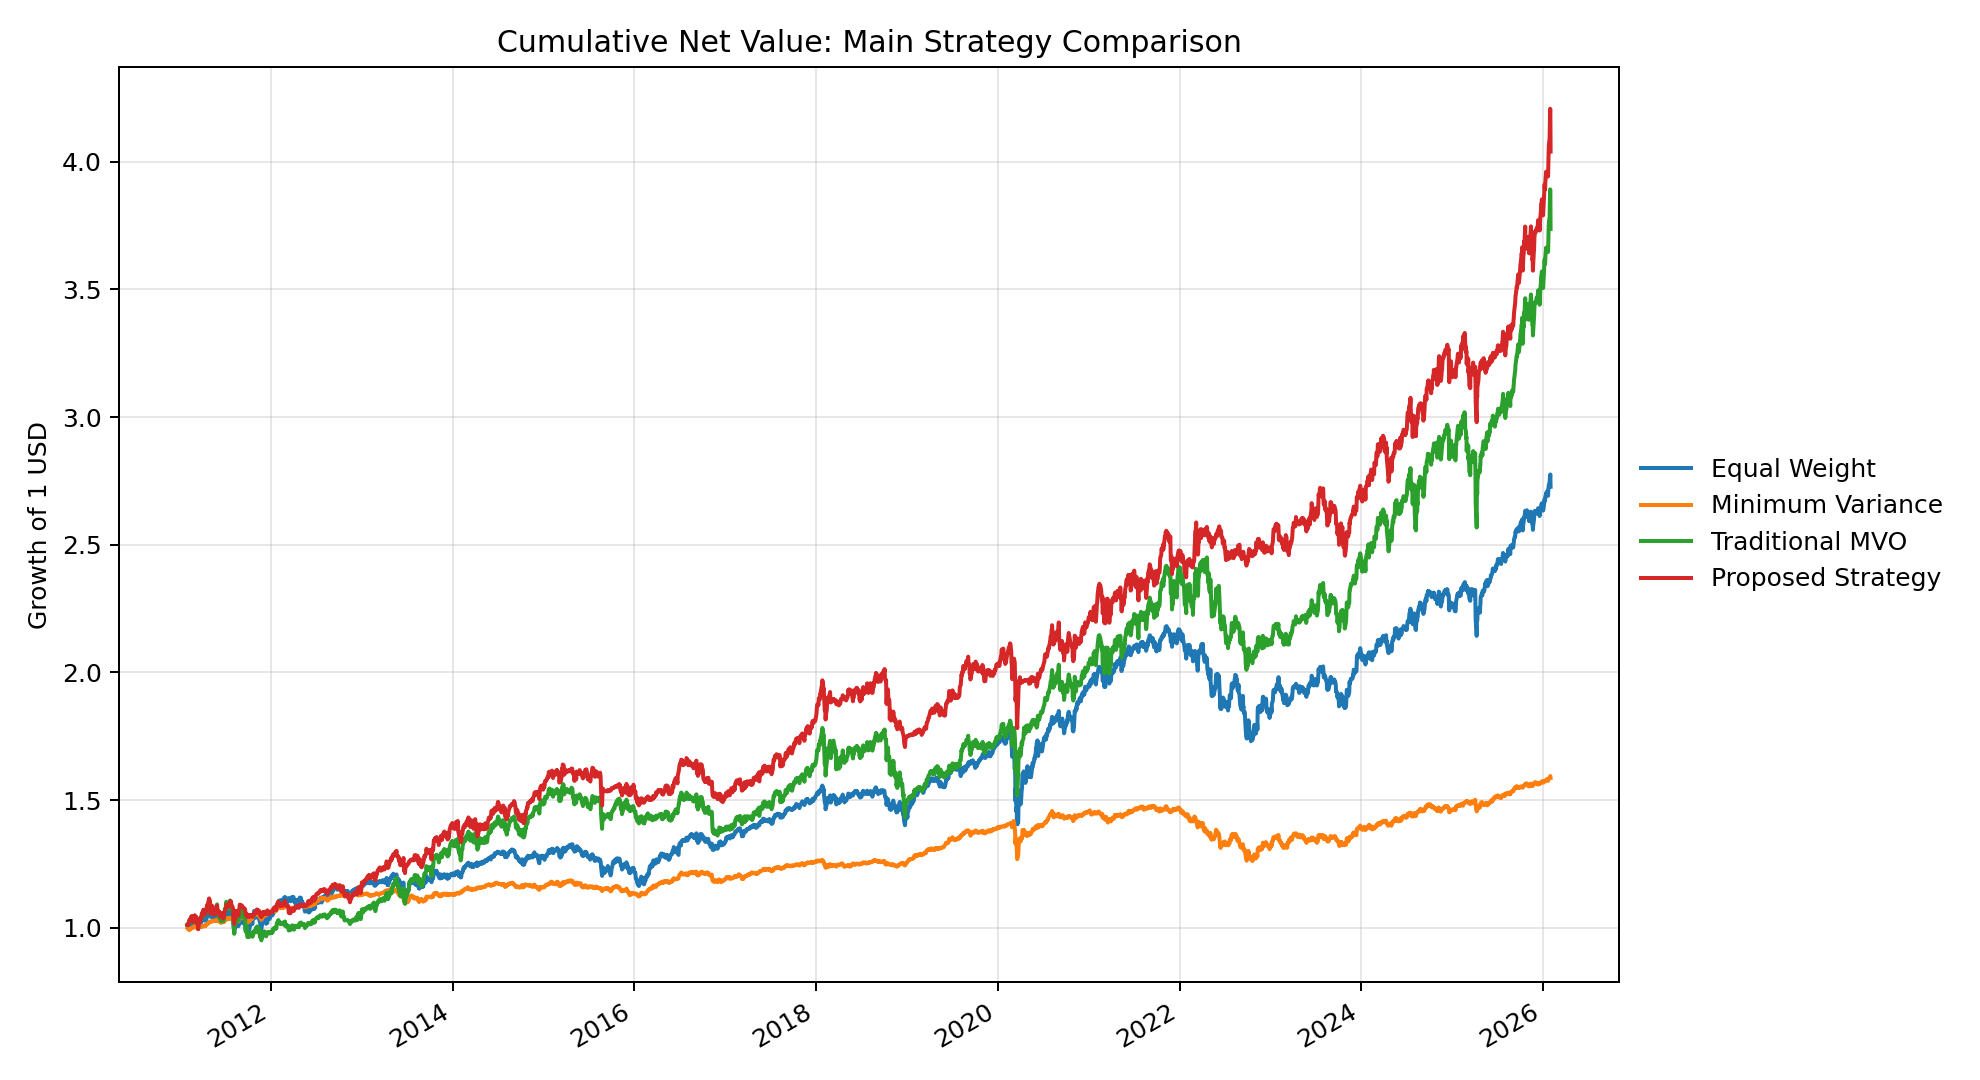
\includegraphics[width=0.94\linewidth]{figure_1_cumulative_net_value.png}
\caption{Cumulative net value for the four final strategies. The figure uses daily net returns after transaction costs and contains only Equal Weight, Minimum Variance, Traditional MVO, and the Proposed Strategy.}
\label{fig:cumulative}
\end{figure}

Figure \ref{fig:cumulative} shows the cumulative net value path. The proposed
strategy compounds more strongly over the full sample, while Traditional MVO also
achieves high terminal wealth but with higher volatility and a larger drawdown. The
comparison should be interpreted jointly with risk and turnover metrics rather than
as a cumulative-return ranking alone.

\subsection{Drawdown Behavior}

\DrawdownSummaryTable

Table \ref{tab:drawdown_summary} and Figure \ref{fig:drawdown} summarize drawdown
behavior. The proposed strategy's maximum drawdown is -15.7\%, occurring from
February 19, 2020 to March 19, 2020 and recovering by July 29, 2020. Equal Weight
and Traditional MVO experience maximum drawdowns of -20.7\% and -19.6\%,
respectively. Minimum Variance has a smaller maximum drawdown of -14.6\%, but its
drawdown period lasts substantially longer. The results indicate that the proposed
strategy reduces drawdown relative to the more return-seeking baselines, while still
remaining exposed to sudden stress periods.

\begin{figure}[!htbp]
\centering
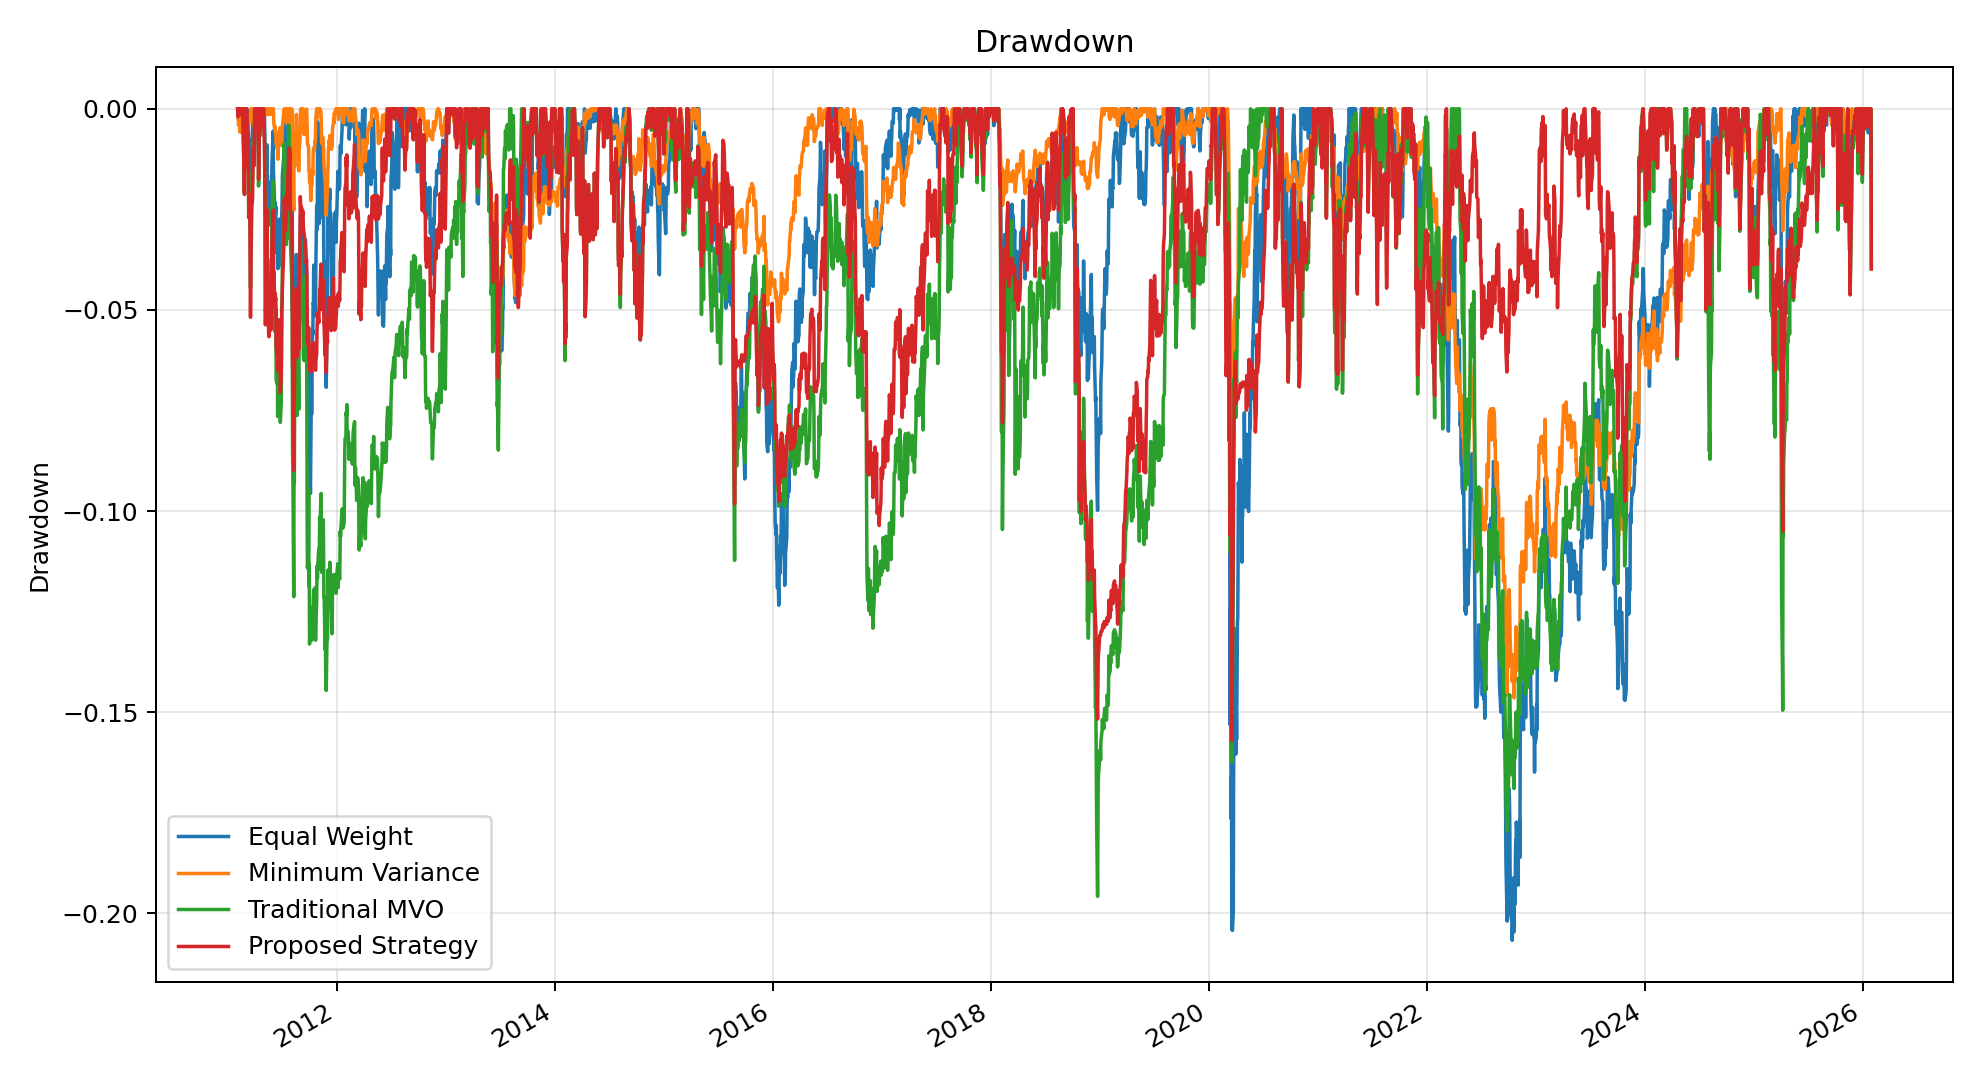
\includegraphics[width=0.84\linewidth]{figure_2_drawdown_curve.png}
\caption{Drawdown curves for the four final strategies. The proposed strategy reduces drawdown relative to Equal Weight and Traditional MVO in the tested sample but does not eliminate drawdown risk.}
\label{fig:drawdown}
\end{figure}

\FloatBarrier

\section{Diagnostic Analysis}
\label{sec:diagnostics}

\subsection{Cash and Exposure Dynamics}

\begin{figure}[!htbp]
\centering
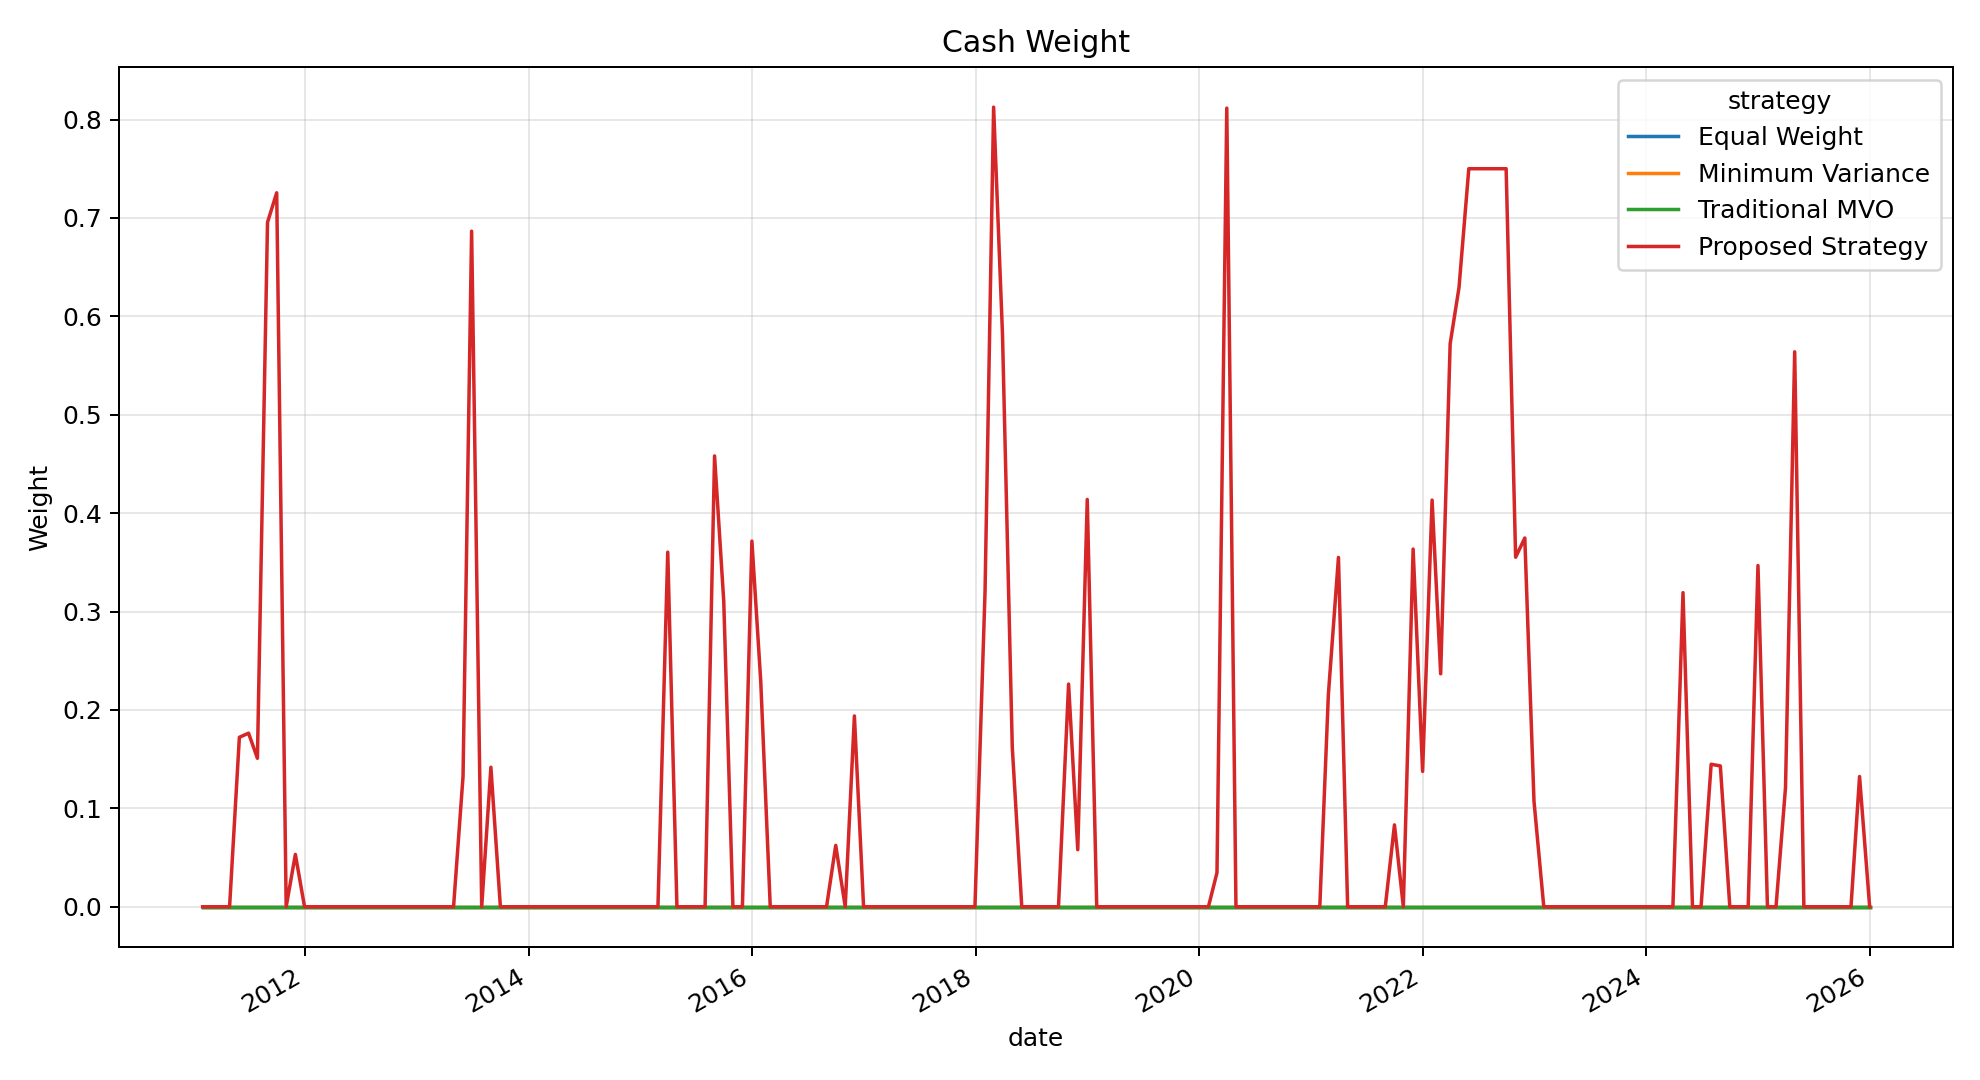
\includegraphics[width=0.84\linewidth]{figure_3_cash_weight.png}
\caption{Cash weight of the proposed strategy. The BIL sleeve allows the optimizer to reduce risky exposure when the forecast-risk tradeoff is unattractive.}
\label{fig:cash}
\end{figure}

Figure \ref{fig:cash} shows that the proposed strategy uses the cash sleeve
meaningfully. The average cash weight is 9.8\%, and the maximum cash weight reaches
81.3\% in the generated exposure summary. This does not mean the model is a pure
market-timing rule; rather, cash is one feasible allocation choice within a
constrained optimization problem.

\begin{figure}[!htbp]
\centering
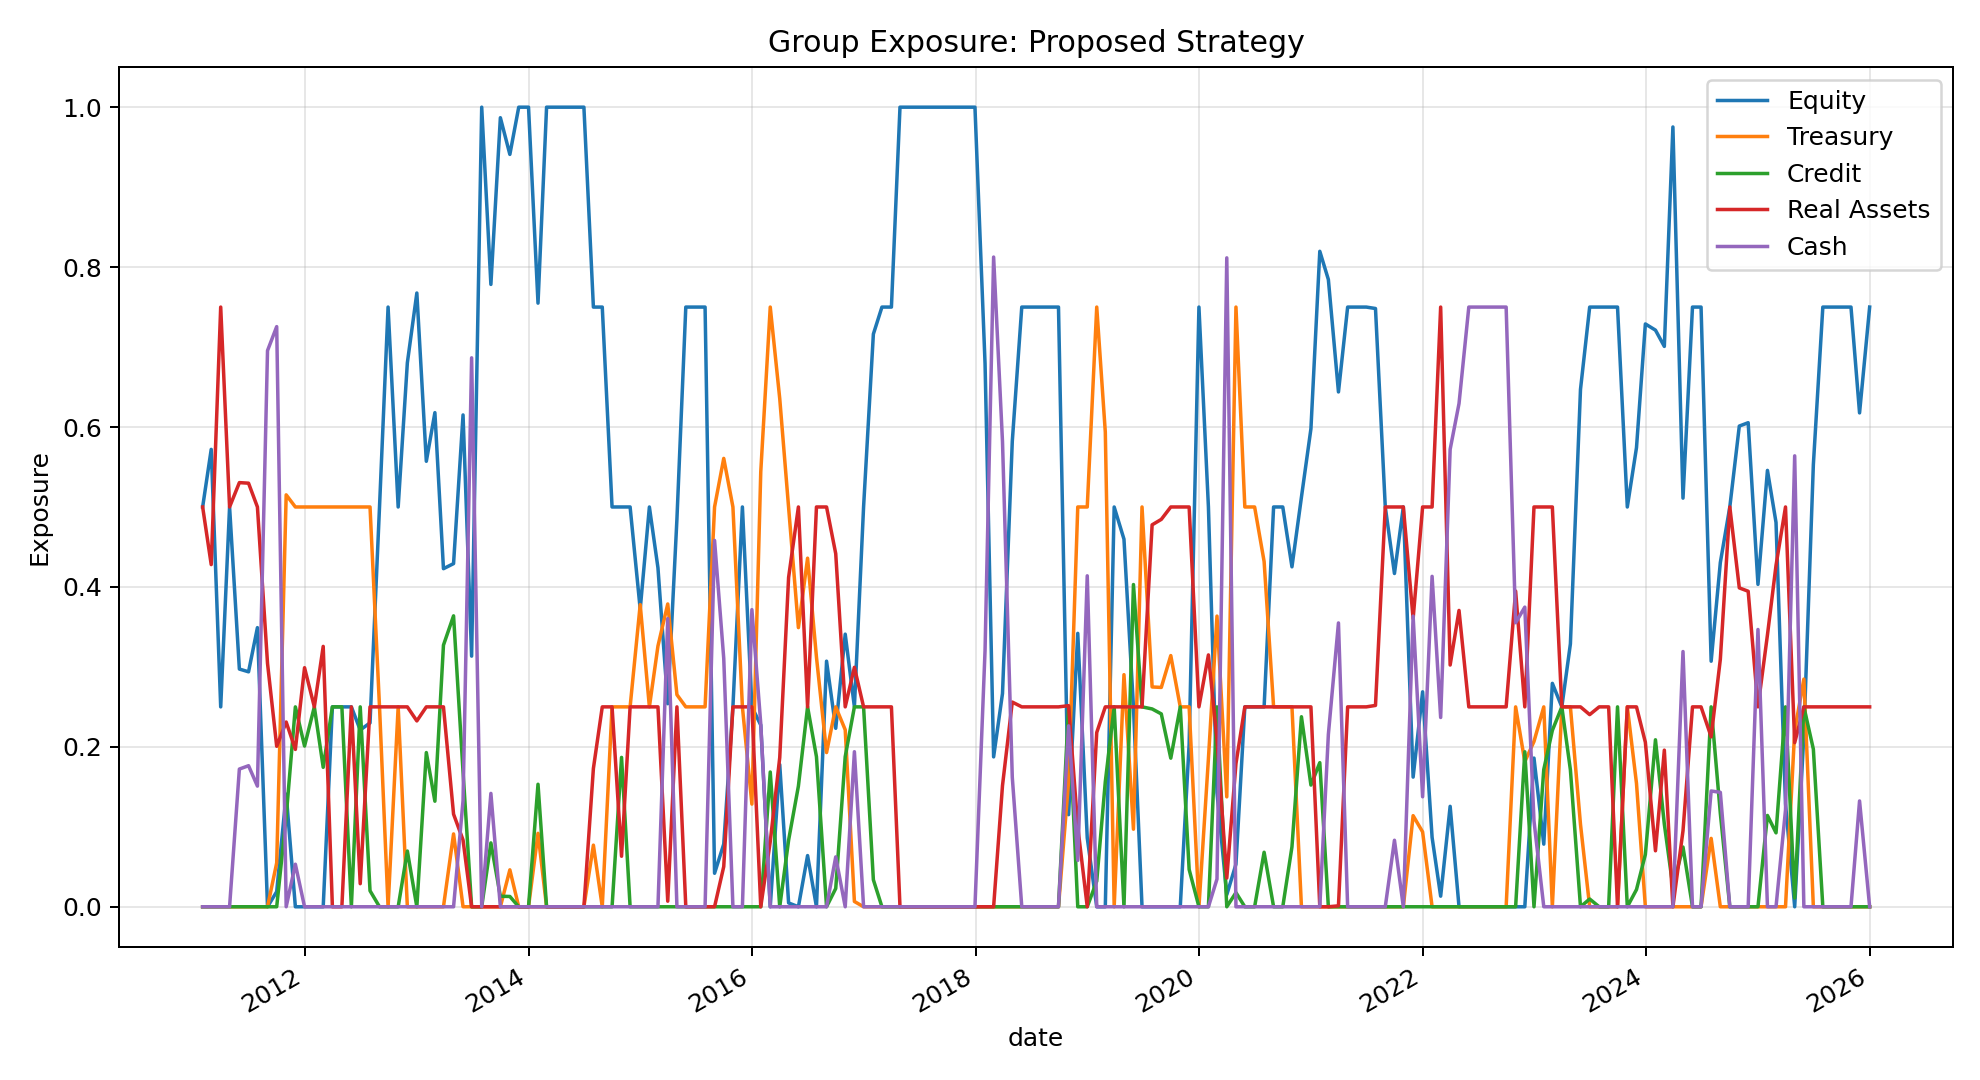
\includegraphics[width=0.84\linewidth]{figure_4_group_exposure.png}
\caption{Group exposures of the proposed strategy. Exposures vary across equity, Treasury, credit, real assets, and cash through the rolling optimization.}
\label{fig:group_exposure}
\end{figure}

Figure \ref{fig:group_exposure} illustrates that the proposed strategy shifts
exposure across asset groups over time. The average risky exposure is 90.2\%, with
average equity exposure of 46.1\%, Treasury exposure of 14.5\%, credit exposure of
6.3\%, and real asset exposure of 23.2\%. During the proposed strategy's maximum
drawdown window, cash exposure is modest, which helps explain why the model still
experiences a meaningful drawdown in the 2020 crash.

\subsection{Risk Forecast Diagnostics}

\begin{figure}[!htbp]
\centering
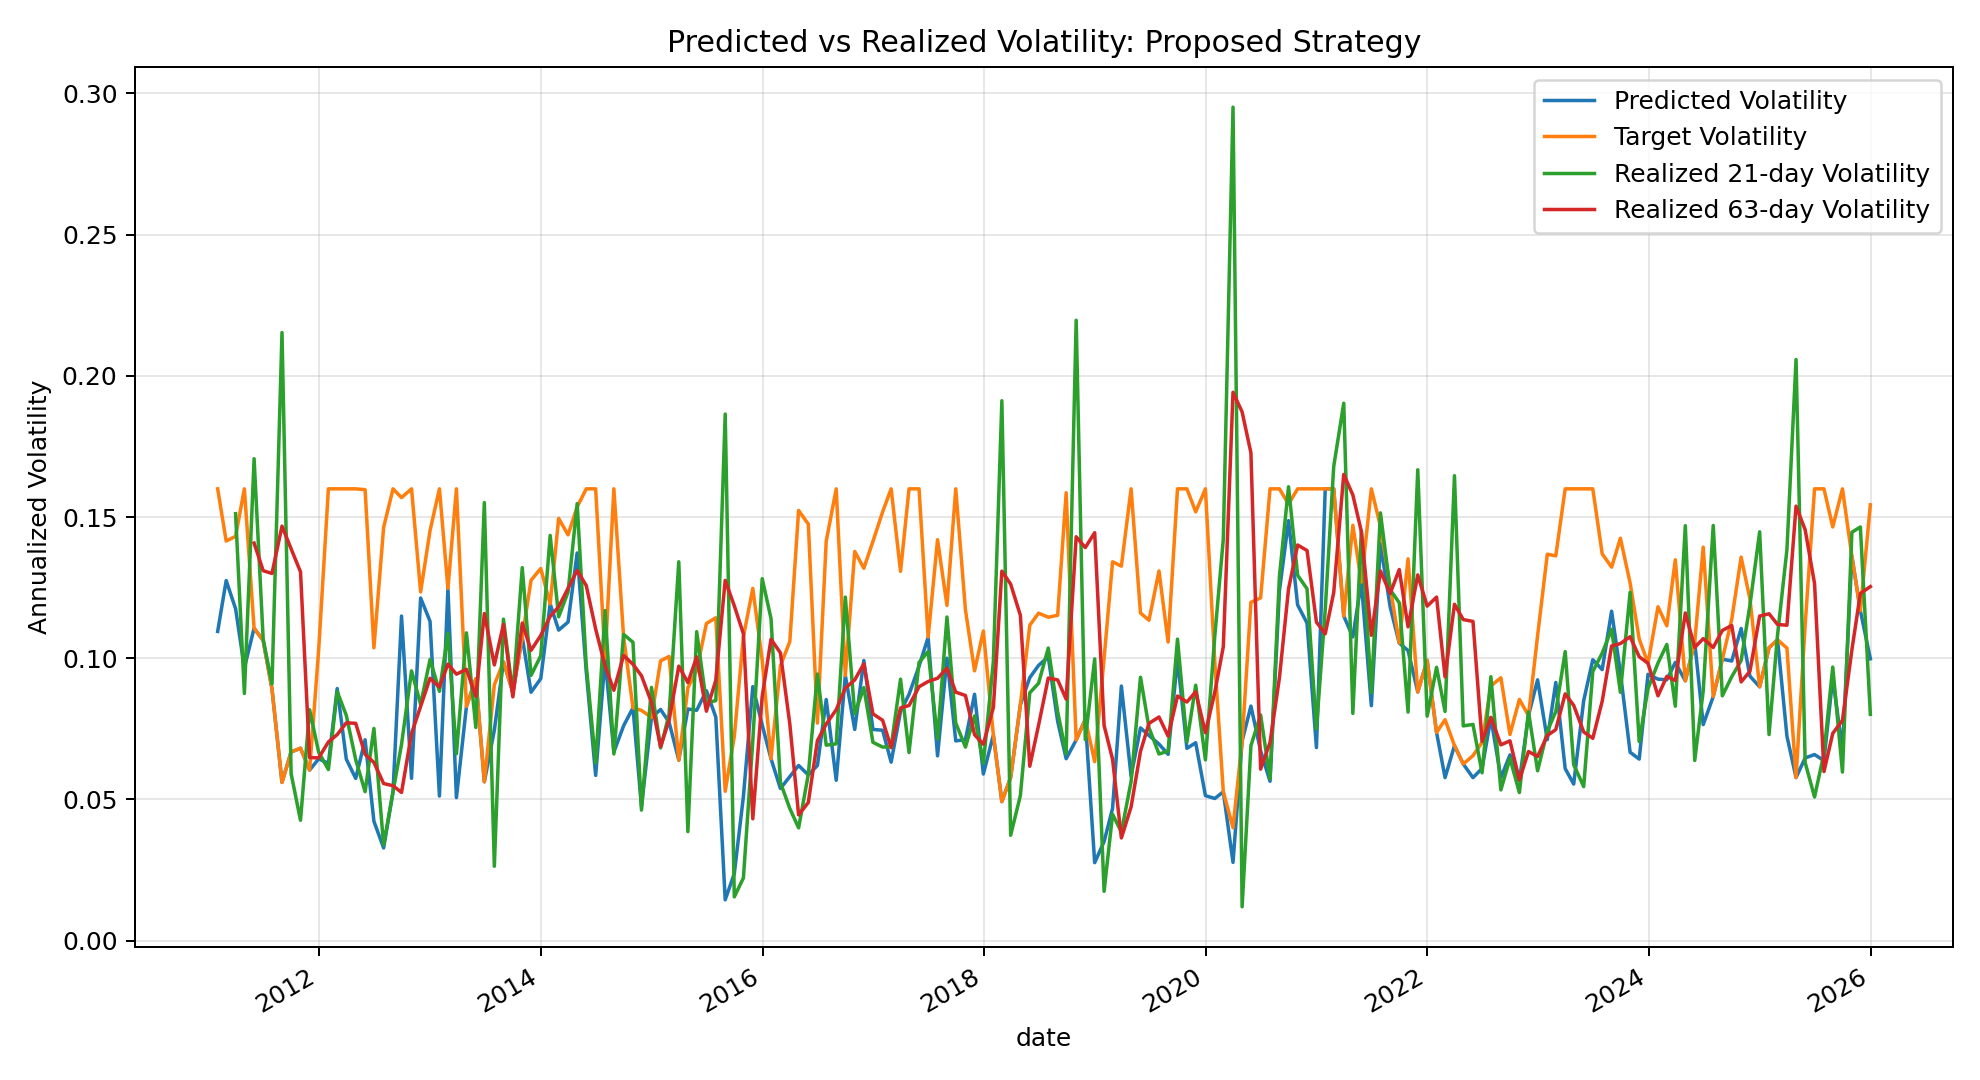
\includegraphics[width=0.86\linewidth]{figure_5_predicted_vs_realized_volatility.png}
\caption{Predicted volatility, dynamic target volatility, and realized volatility for the proposed strategy. Realized volatility can exceed predicted volatility during stress periods.}
\label{fig:risk_forecast}
\end{figure}

\SignalRiskDiagnosticsTable

The risk diagnostics in Table \ref{tab:signal_risk_diagnostics} and Figure
\ref{fig:risk_forecast} show that the model's average predicted volatility is 8.2\%,
while average realized 21-day volatility is 9.3\% and average realized 63-day
volatility is 9.8\%. The average realized-to-predicted volatility ratio is 1.28, and
the maximum ratio is much larger during stress. This indicates that the EWMA risk
model is responsive but can still underestimate future realized risk in abrupt
market moves. The target-volatility constraint binds in 28.3\% of rebalance periods,
so the risk budget is active but not always the dominant constraint.

\subsection{Signal Diagnostics}

\begin{figure}[!htbp]
\centering
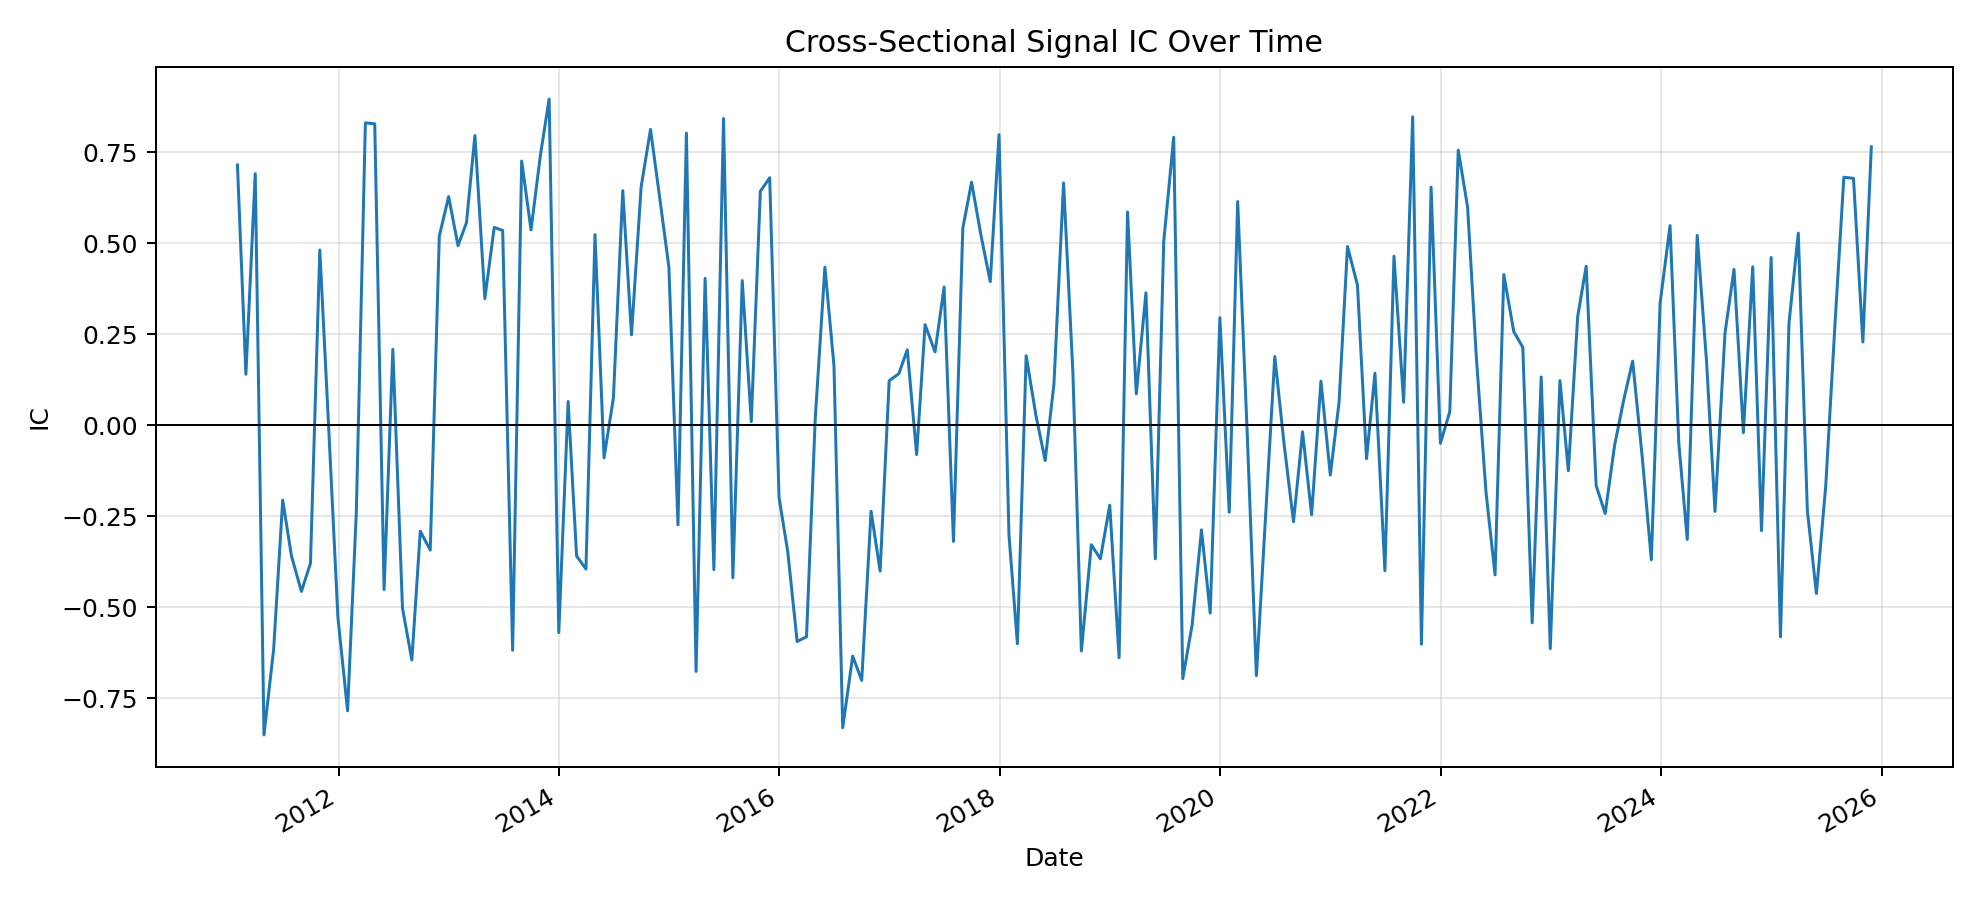
\includegraphics[width=0.84\linewidth]{figure_6_signal_ic_over_time.png}
\caption{Monthly cross-sectional information coefficient of the forecast signal. The signal is positive on average but noisy across rebalance periods.}
\label{fig:signal_ic}
\end{figure}

The average cross-sectional information coefficient is 0.072 with a t-statistic of
2.11 and a positive IC ratio of 55.3\%. The signal is stronger in normal periods
than during drawdowns: average IC is 0.088 in normal periods and 0.015 in drawdown
periods. These diagnostics support a cautious interpretation. The momentum and trend
signal appears informative on average in the tested sample, but its predictive power
is far from stable, particularly during adverse market regimes.

\subsection{Turnover and Transaction Costs}

\begin{figure}[!htbp]
\centering
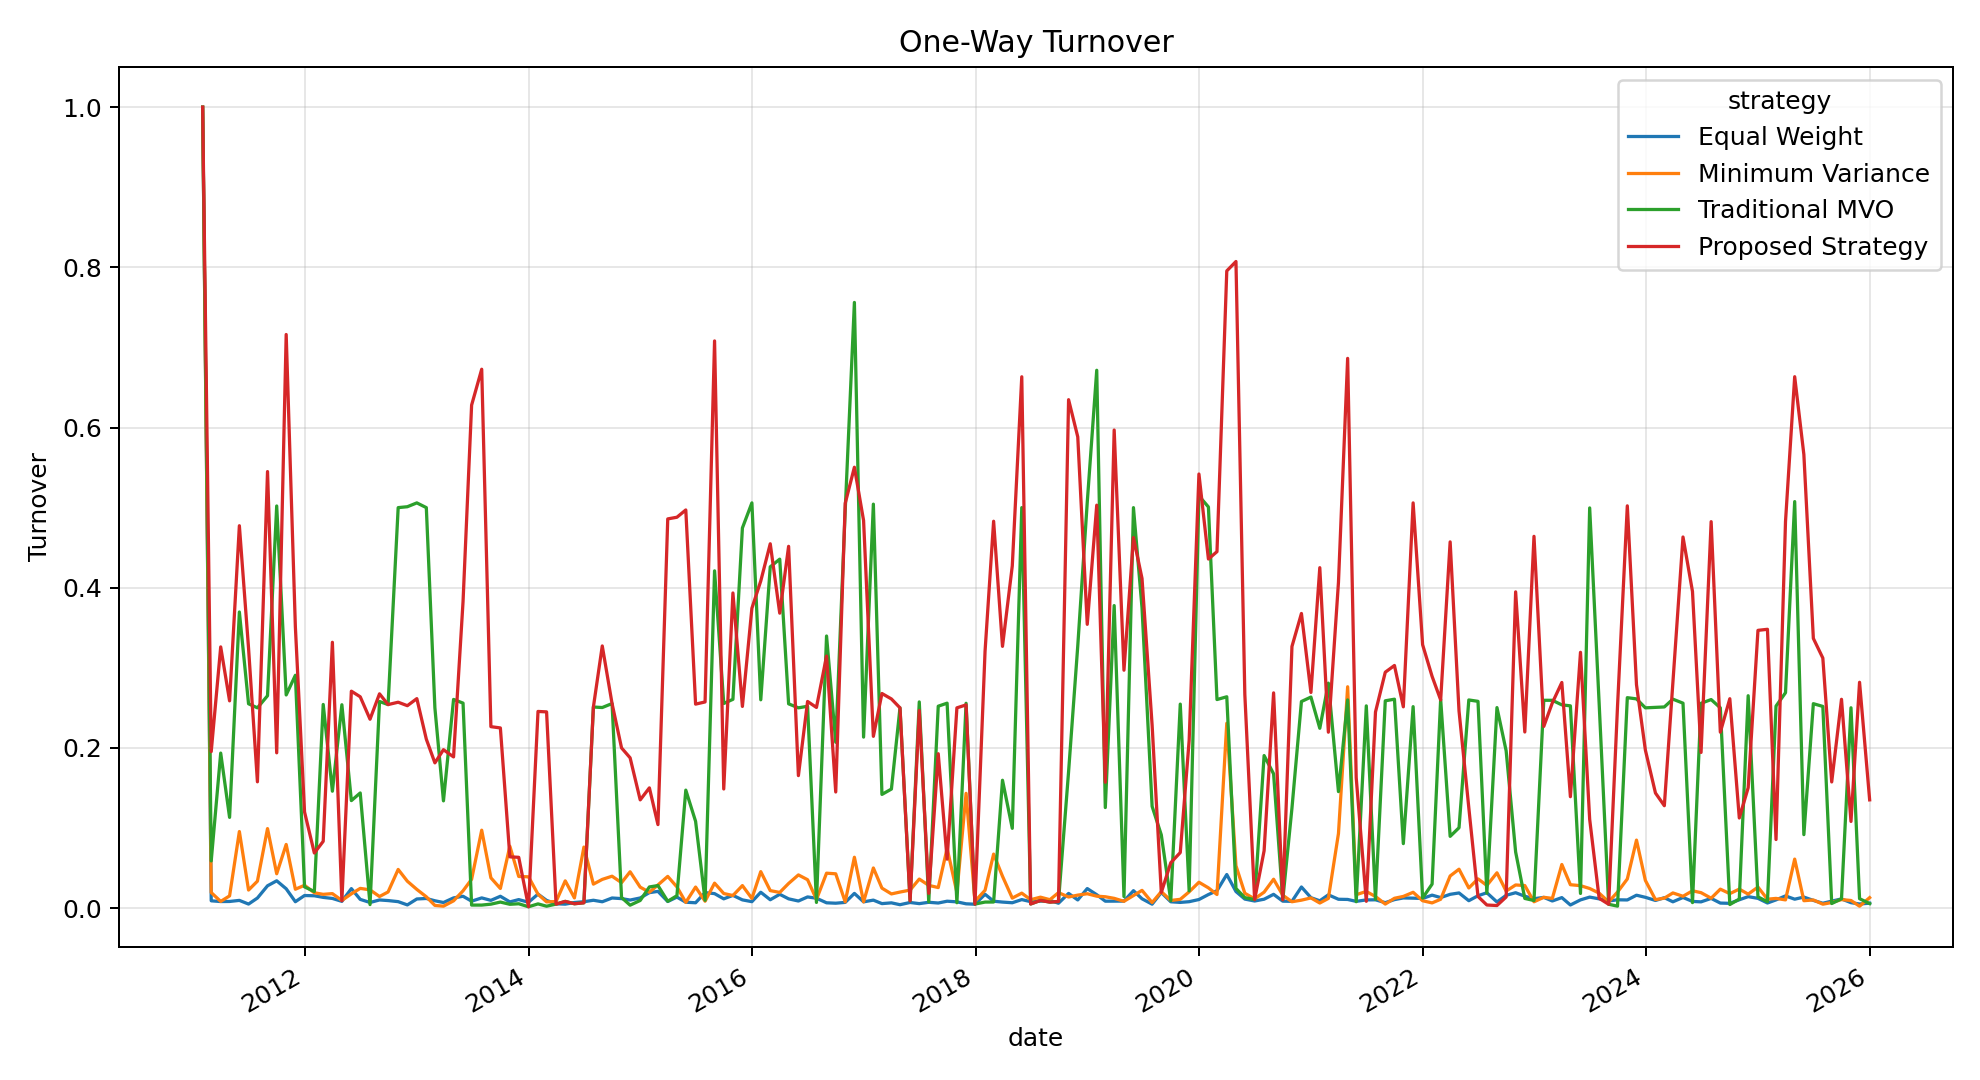
\includegraphics[width=0.86\linewidth]{figure_8_turnover_over_time.png}
\caption{One-way turnover over time. Turnover is computed using the full vector, including the BIL cash sleeve for the proposed strategy.}
\label{fig:turnover}
\end{figure}

The proposed strategy has average one-way turnover of 27.7\%, higher than the three
baselines. At a 10 bps one-way transaction cost rate, its annualized transaction-cost
drag is 0.37\%, and its final gross value of 4.25 is reduced to a final net value of
4.04. Transaction costs therefore matter, but they do not fully explain the
difference between the proposed strategy and the baselines in this sample.

\FloatBarrier

\section{Robustness Analysis}
\label{sec:robustness}

The sensitivity tests are used to examine parameter dependence rather than to select
parameters in sample. The final proposed strategy remains the fixed specification
defined in Section \ref{sec:methodology}.

\TargetVolSensitivityTable

Table \ref{tab:target_vol_sensitivity} shows that lower base target-volatility
settings increase average cash weight and reduce drawdown, while higher settings
increase risky exposure. The 10\% setting used in the final model is not selected by
ex post performance maximization; it is the fixed specification used for the main
backtest.

\begin{figure}[!htbp]
\centering
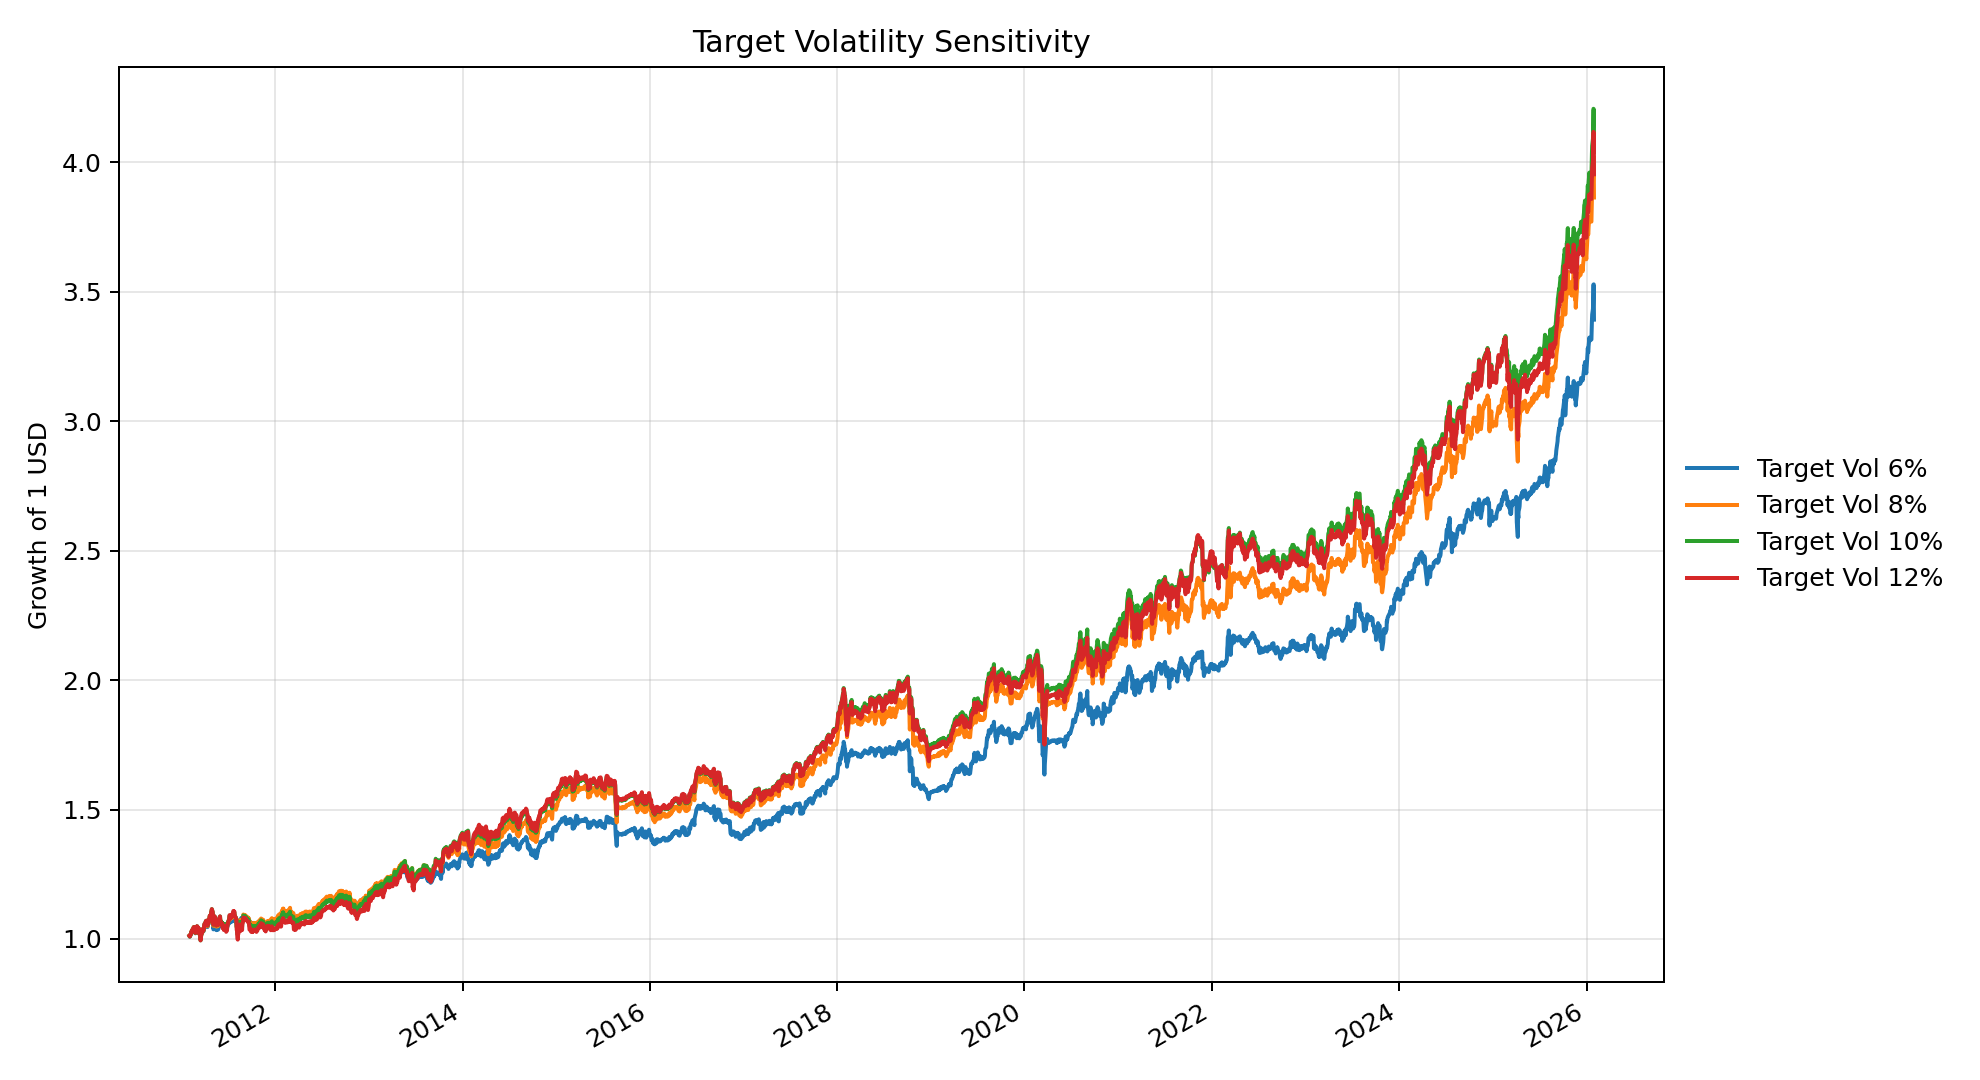
\includegraphics[width=0.86\linewidth]{figure_7_target_vol_sensitivity.png}
\caption{Target-volatility sensitivity for the proposed strategy. The grid changes the base risk budget while preserving the same signal and robust optimization structure.}
\label{fig:target_sensitivity}
\end{figure}

\AlphaScaleSensitivityTable

Table \ref{tab:alpha_scale_sensitivity} varies the alpha scale. Larger alpha scale
generally increases return but also increases drawdown and slightly reduces cash
allocation. This is consistent with the interpretation that the alpha signal is
useful but noisy: giving it too much weight can increase exposure to forecast error.

\RhoSensitivityTable

Table \ref{tab:rho_sensitivity} shows that increasing the robust penalty tends to
raise cash allocation and reduce maximum drawdown, at the cost of lower annualized
return in this sample. The case with zero robust penalty is reported only as a
sensitivity test, not as a main baseline.

\CovarianceSensitivityTable

Table \ref{tab:covariance_sensitivity} compares covariance estimators. Ledoit-Wolf
shrinkage performs well in this sensitivity table, but it is not the implemented
final risk model. The final specification uses the 20-day EWMA covariance estimator
because it reflects the chosen short-horizon risk-control design. The comparison
also shows that conclusions can be sensitive to covariance estimation, which is an
important limitation.

\TransactionCostSensitivityTable

Table \ref{tab:transaction_cost_sensitivity} confirms that higher transaction costs
reduce net performance. Moving from zero costs to 25 bps lowers annualized return
from 10.1\% to 9.2\% and final net value from 4.25 to 3.75. The model remains
economically reasonable under the tested cost grid, but a more detailed market-impact
model could change this assessment.

Subperiod results further show that performance is regime-dependent. During the 2022
stock-bond drawdown, the proposed strategy loses 9.8\% annualized with a -6.5\%
maximum drawdown, compared with larger drawdowns for Equal Weight and Traditional
MVO. During the COVID crash and recovery period, however, the proposed strategy's
Sharpe ratio is only 0.21 and its maximum drawdown is -15.7\%, illustrating that
fast crashes remain difficult for the risk model to avoid.

\section{Implementation Checks}
\label{sec:checks}

\ImplementationChecksTable

Table \ref{tab:implementation_checks} reports numerical feasibility and timing
checks. The maximum target-volatility violation is below \(5\times10^{-10}\), there
are no solver failures or fallback uses, and all five timing checks pass. The timing
checks verify that signals and covariances are computed using information available
no later than the rebalance date, that weights are applied only after the rebalance
date, and that BIL is excluded from alpha and covariance construction.

\section{Discussion and Limitations}
\label{sec:discussion}

The results suggest that robust forecast-aware optimization can improve certain
risk-adjusted metrics relative to the selected baselines in the tested sample. The
framework is interpretable: alpha comes from momentum and trend signals, risk comes
from EWMA covariance estimation with PSD repair, robustness is represented by an
ellipsoidal alpha-uncertainty penalty, and cash enters through an explicit BIL
sleeve. The model is also implementable because it is a convex optimization problem
with transparent constraints and explicit transaction-cost accounting.

Several limitations are important. First, expected-return forecasts remain noisy.
The signal diagnostics show positive average IC, but also substantial time variation
and weaker performance during drawdown periods. Second, covariance forecasts can
underestimate realized risk in sudden crises. The realized-to-predicted volatility
ratio indicates that the EWMA estimator is not a complete solution to risk-forecast
error. Third, the transaction-cost model is simplified. It accounts for full-vector
turnover at a constant one-way cost rate, but does not model bid-ask spread
differences across ETFs, taxes, market impact, or liquidity-dependent slippage.

The results also depend on the ETF universe, sample period, and fixed parameter
choices. Parameters such as \(\alpha_{scale}\), \(\rho_t\), the EWMA decay, and the
target-risk bounds are economically motivated but partly heuristic. The paper does
not claim that the proposed strategy is optimal in real markets or that it will
outperform in future periods. Future work could study alternative covariance
forecasting models, richer transaction-cost models, alternative cash proxies,
international ETF universes, and formal drawdown-aware optimization as an extension.
The final model in this paper, however, does not use any drawdown-based rebalancing
trigger.

\section{Conclusion}
\label{sec:conclusion}

This paper studies a cash-allowed robust forecast-aware optimization framework for
multi-asset ETF allocation. The model combines momentum and trend forecasts,
annualized 20-day EWMA covariance estimation with PSD repair, a robust forecast
uncertainty penalty, a dynamic target-risk budget, full-vector turnover costs, and a
BIL cash sleeve. The framework is evaluated through monthly rolling out-of-sample
backtests against Equal Weight, Minimum Variance, and Traditional MVO baselines.

In the tested sample, the proposed strategy achieves the highest final net value and
the highest Sharpe ratio among the four strategies. It also reduces maximum drawdown
relative to Equal Weight and Traditional MVO, though not relative to Minimum
Variance. Diagnostic results show that the signal has positive but noisy
cross-sectional predictive content, the cash sleeve is used meaningfully, and the
risk model can still underestimate realized volatility during abrupt stress events.

Overall, the evidence suggests that robust forecast-aware optimization with an
explicit cash sleeve provides a useful and interpretable framework for multi-asset
ETF allocation. The results should be interpreted with caution because the model
remains exposed to forecast uncertainty, covariance estimation error, transaction
cost assumptions, and regime changes.

\appendix

\section{Methodology-Code Consistency}

\MethodologyCodeConsistencyTable

\section{References}

\begin{thebibliography}{}

\bibitem[Asness et~al., 2013]{asness2013}
Asness, C.~S., Moskowitz, T.~J., and Pedersen, L.~H. (2013).
\newblock Value and momentum everywhere.
\newblock \emph{The Journal of Finance}, 68(3):929--985.

\bibitem[Barroso and Santa-Clara, 2015]{barroso2015}
Barroso, P. and Santa-Clara, P. (2015).
\newblock Momentum has its moments.
\newblock \emph{Journal of Financial Economics}, 116(1):111--120.

\bibitem[Boyd et~al., 2017]{boyd2017}
Boyd, S., Busseti, E., Diamond, S., Kahn, R.~N., Koh, K., Nystrup, P., and Speth, J. (2017).
\newblock Multi-period trading via convex optimization.
\newblock \emph{Foundations and Trends in Optimization}, 3(1):1--76.

\bibitem[DeMiguel et~al., 2009]{demiguel2009}
DeMiguel, V., Garlappi, L., and Uppal, R. (2009).
\newblock Optimal versus naive diversification: How inefficient is the 1/N portfolio strategy?
\newblock \emph{The Review of Financial Studies}, 22(5):1915--1953.

\bibitem[Faber, 2007]{faber2007}
Faber, M.~T. (2007).
\newblock A quantitative approach to tactical asset allocation.
\newblock \emph{The Journal of Wealth Management}, 9(4):69--79.

\bibitem[Goldfarb and Iyengar, 2003]{goldfarbiyengar2003}
Goldfarb, D. and Iyengar, G. (2003).
\newblock Robust portfolio selection problems.
\newblock \emph{Mathematics of Operations Research}, 28(1):1--38.

\bibitem[Harvey et~al., 2018]{harvey2018}
Harvey, C.~R., Hoyle, E., Korgaonkar, R., Rattray, S., Sargaison, M., and Van Hemert, O. (2018).
\newblock The impact of volatility targeting.
\newblock \emph{The Journal of Portfolio Management}, 45(1):14--33.

\bibitem[Jagannathan and Ma, 2003]{jagannathanma2003}
Jagannathan, R. and Ma, T. (2003).
\newblock Risk reduction in large portfolios: Why imposing the wrong constraints helps.
\newblock \emph{The Journal of Finance}, 58(4):1651--1683.

\bibitem[Ledoit and Wolf, 2004]{ledoitwolf2004}
Ledoit, O. and Wolf, M. (2004).
\newblock Honey, I shrunk the sample covariance matrix.
\newblock \emph{The Journal of Portfolio Management}, 30(4):110--119.

\bibitem[Markowitz, 1952]{markowitz1952}
Markowitz, H. (1952).
\newblock Portfolio selection.
\newblock \emph{The Journal of Finance}, 7(1):77--91.

\bibitem[Moreira and Muir, 2017]{moreira2017}
Moreira, A. and Muir, T. (2017).
\newblock Volatility-managed portfolios.
\newblock \emph{The Journal of Finance}, 72(4):1611--1644.

\bibitem[Moskowitz et~al., 2012]{moskowitz2012}
Moskowitz, T.~J., Ooi, Y.~H., and Pedersen, L.~H. (2012).
\newblock Time series momentum.
\newblock \emph{Journal of Financial Economics}, 104(2):228--250.

\end{thebibliography}

\end{document}
